\chapter{The dashboard: a guided tour}
\label{ch:ui}

Use this part to rehearse the demo. For each page: what it shows, what to point at, and one sentence to say.

\section{The sidebar and the top bar}
\begin{simplebox}
On the left there is a menu with the pages. In the top bar you pick a project (or ``All projects''), see how many services are healthy, degraded or critical, and use the \textbf{Rules / Hybrid / ML} switch. At the right there is a green ``Live'' light and the time of the last update. While a project is still learning its normal behaviour the bar says ``Learning baseline, 5 of 30 min''. That is honest: for the first thirty minutes a project has no learned rule model, and only container facts (a stopped container) can raise incidents.
\end{simplebox}

\begin{techbox}
Pages: \emph{Incidents \& cascade}, \emph{Detection engines}, \emph{Cascade risk}, \emph{Spatial view} (3D), \emph{Architecture} (2D), \emph{Telemetry}, \emph{Traces}, \emph{Dependencies}, \emph{Analytics}. Three research pages (ML pipeline, model findings from the optional Python sidecar, experiment history) are hidden until the operator switches them on under ``Show research tools''. The setting \code{MAPPER\_BASELINE\_MIN} (30) controls the learning period.
\end{techbox}

\section{Architecture (2D)}
\begin{figure}[H]
\centering
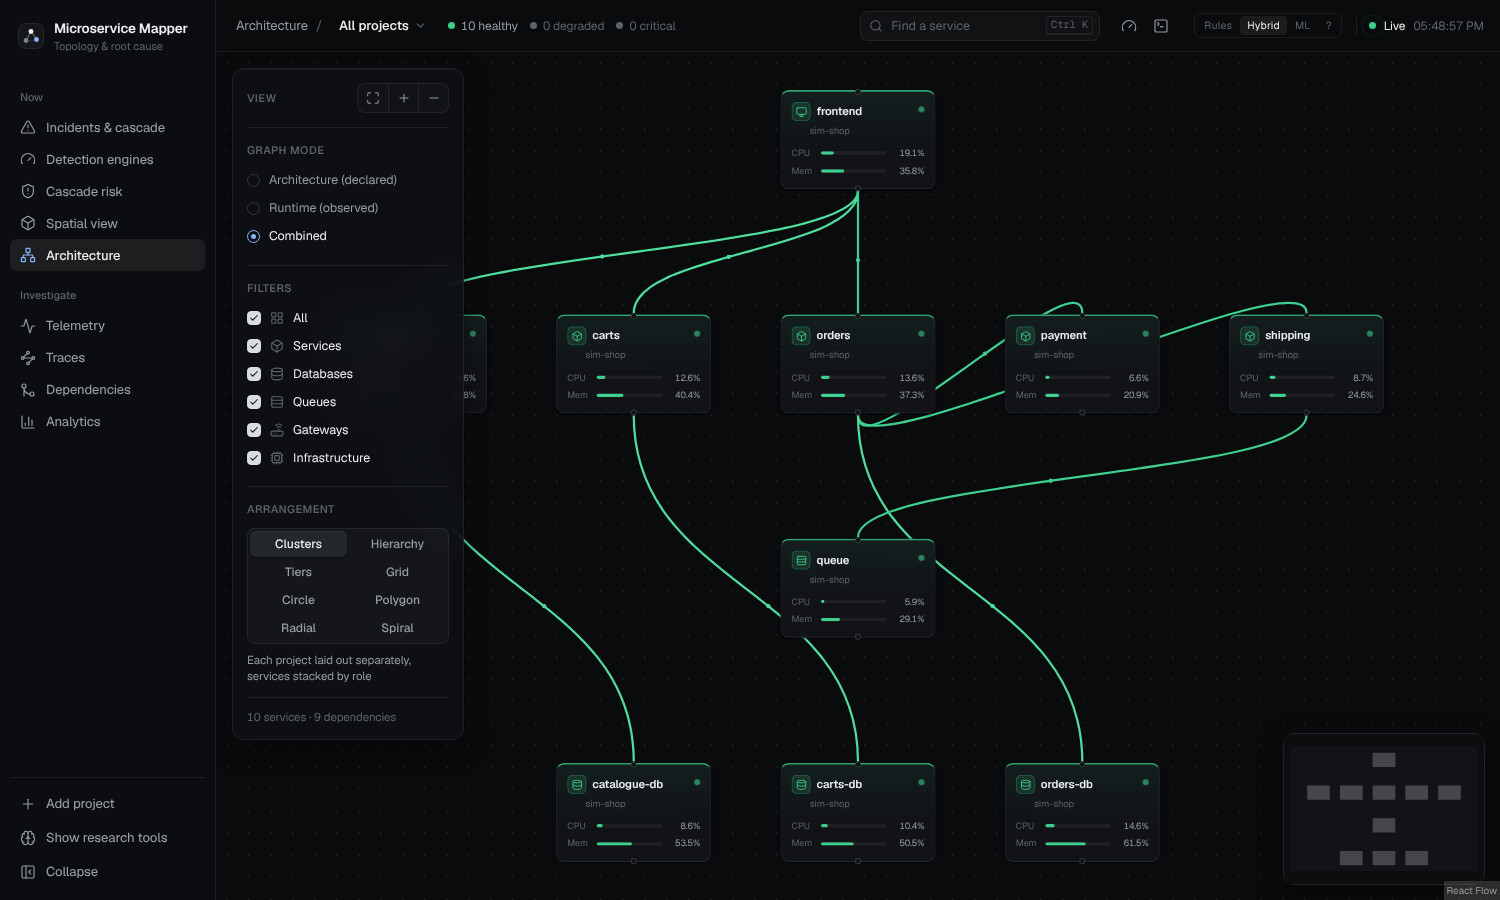
\includegraphics[width=0.96\textwidth]{ui_architecture.jpg}
\caption{The 2D dependency graph with arrangement and filter controls.}
\end{figure}
\begin{simplebox}
The flat map of services as boxes joined by lines. Each box shows CPU and memory against the container's own allowance. Lines show dependencies, and when we have actually seen traffic on them, their activity. You can choose different layouts (clusters, hierarchy, tiers, grid, circle, radial, spiral).
\end{simplebox}
\begin{saybox}
``This is the map the rest of the system works on. Declared and observed links are both shown; observed ones carry evidence.''
\end{saybox}

\section{Incidents and cascade}
\begin{figure}[H]
\centering
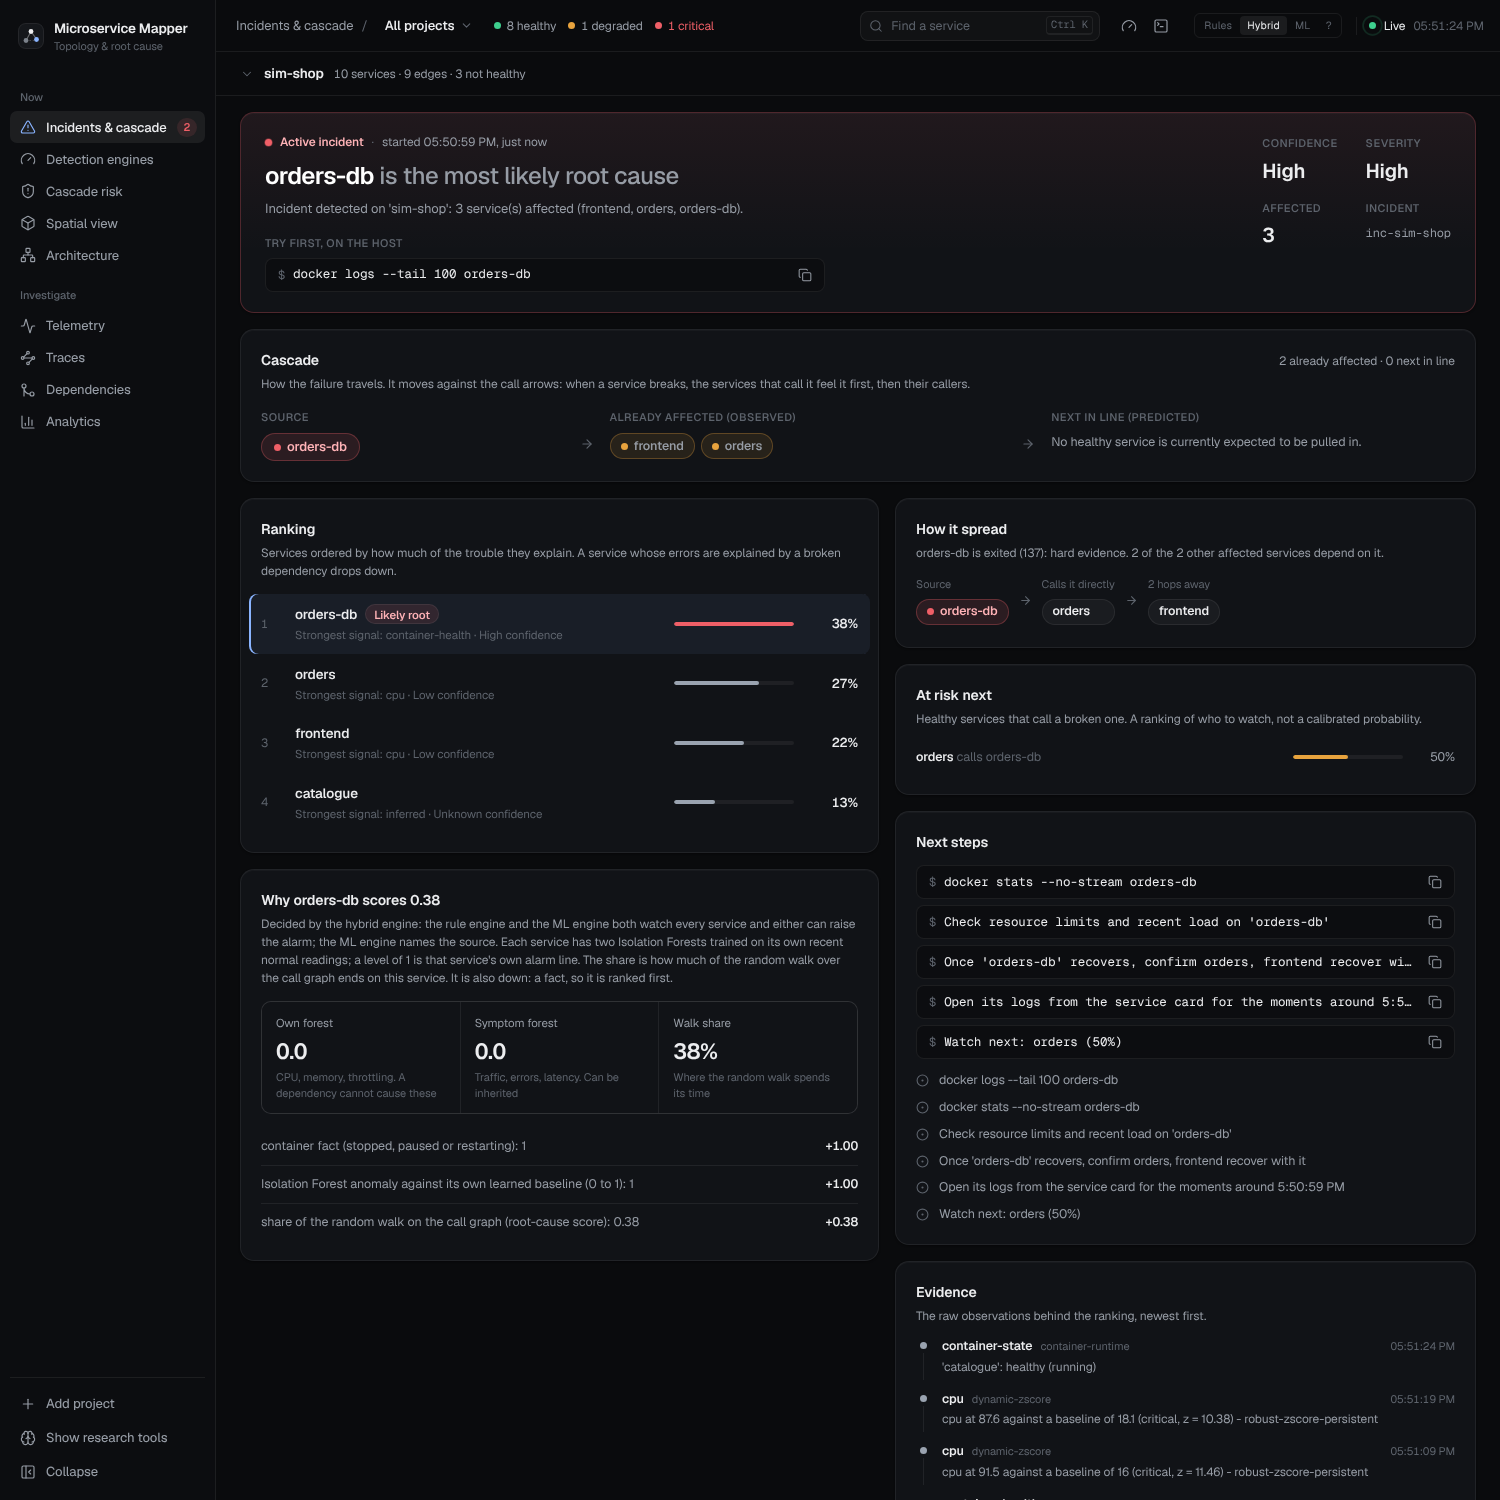
\includegraphics[width=0.78\textwidth]{ui_incident_active.png}
\caption{An active incident after \code{orders-db} was killed.}
\end{figure}
\begin{simplebox}
When something goes wrong, this page opens an incident. At the top: the most likely root cause, how confident the tool is, and how severe. Below that: a \emph{cascade panel} with three groups --- the source, the services already affected, and the services predicted to be next. A \emph{ranking} lists each service with the strongest signal behind its score. A \emph{Why} panel splits a score into its own, symptom and walk parts, and lists the evidence. At the bottom, \emph{next steps}: concrete commands to run on the host.
\end{simplebox}
\begin{saybox}
``Read it top to bottom: who, how sure, who is hurt, who is next, why, and what to do. Every number has a parts breakdown you can open.''
\end{saybox}

\section{Detection engines (the page for the ML story)}
\begin{figure}[H]
\centering
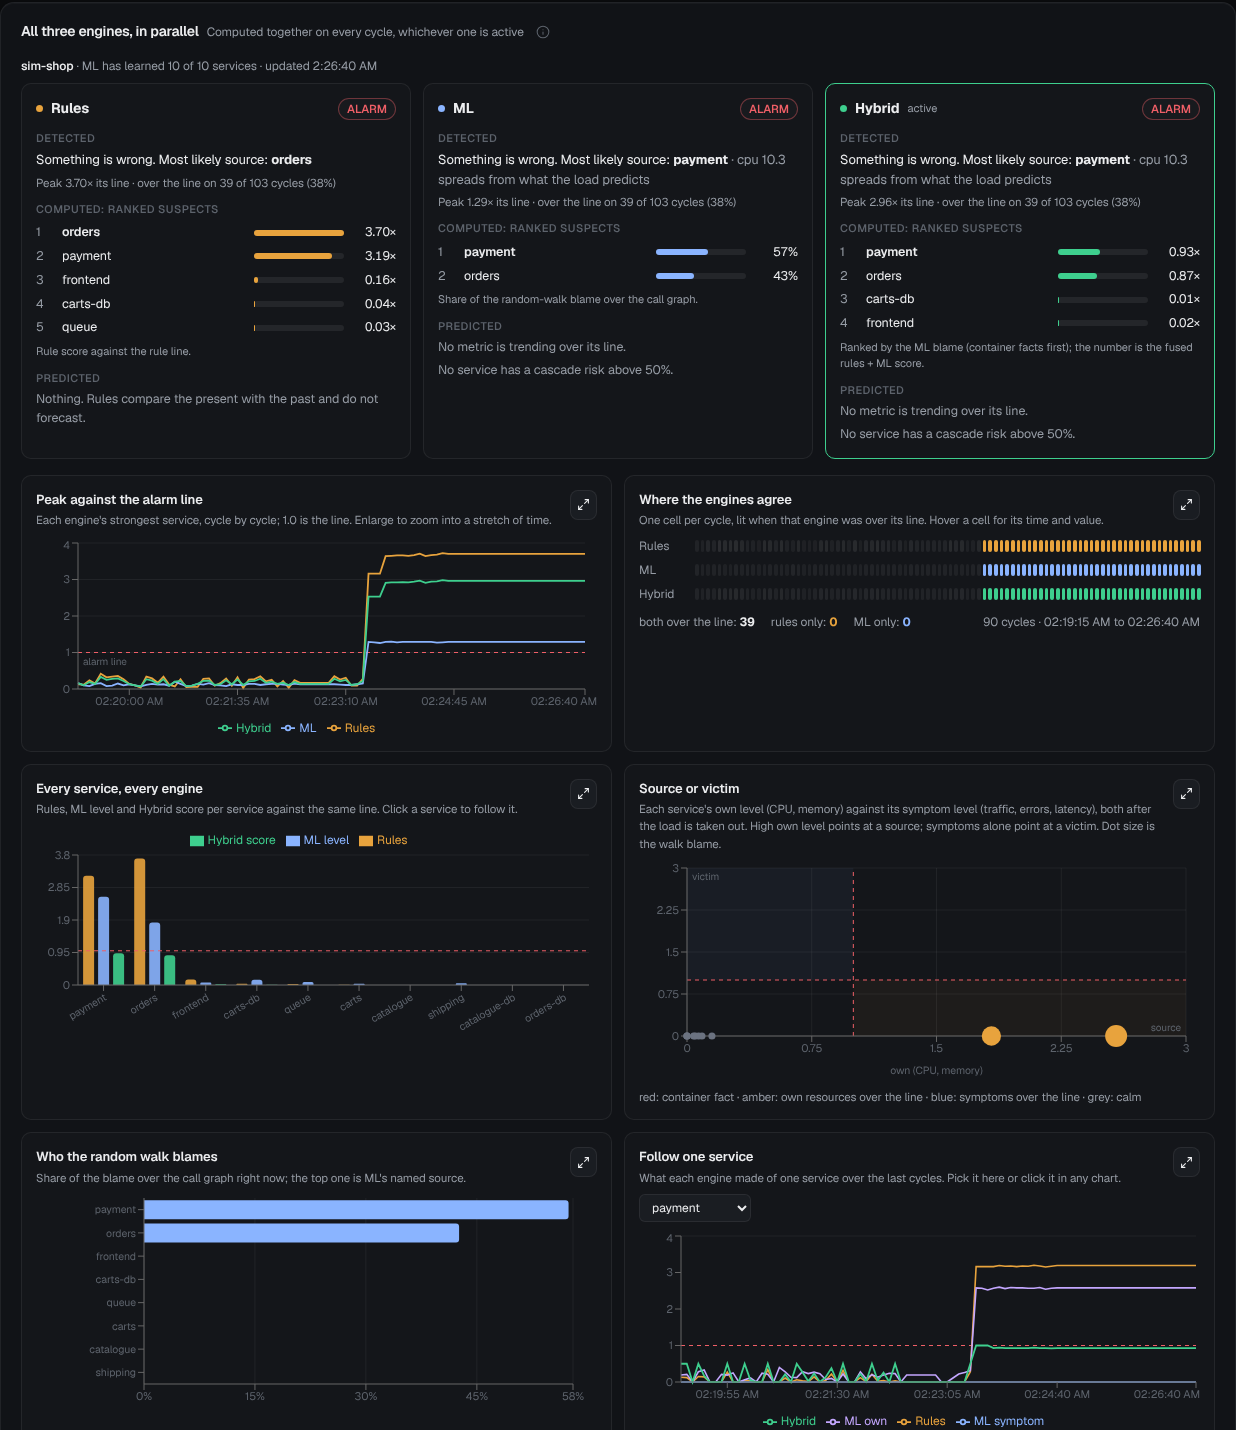
\includegraphics[width=0.92\textwidth,height=0.78\textheight,keepaspectratio]{ui_engines_alarm.png}
\caption{The Detection engines page during a slow-payment fault.}
\end{figure}
\begin{simplebox}
This is the page to use when you explain the ML correction. The top explains Rules, ML and Hybrid in four short lines each. The three middle columns show \emph{what each engine thinks right now about the same data}. In the screenshot, Rules blame \code{orders} (the louder victim); ML and Hybrid name \code{payment} and say \emph{why} (``cpu 10.3 spreads from what the load predicts''). A small chip beside the project name says whether the shared workload moved. Below are six charts; each has a button that enlarges it into a pop-up with a brush for zooming into a few seconds of time.
\end{simplebox}

\begin{techbox}
Charts: each engine's peak against its alarm line; a strip showing the cycles on which the engines agreed; the level of every service under every engine; a source-or-victim scatter (own resources against symptoms); the share of blame from the random walk; a trail for one chosen service. The page ends with the configuration of both engines in plain words (alarm line 4 spreads, alarm level 2, persistence 2 windows, window 120, slow reference 360 readings, and so on).
\end{techbox}

\begin{figure}[H]
\centering
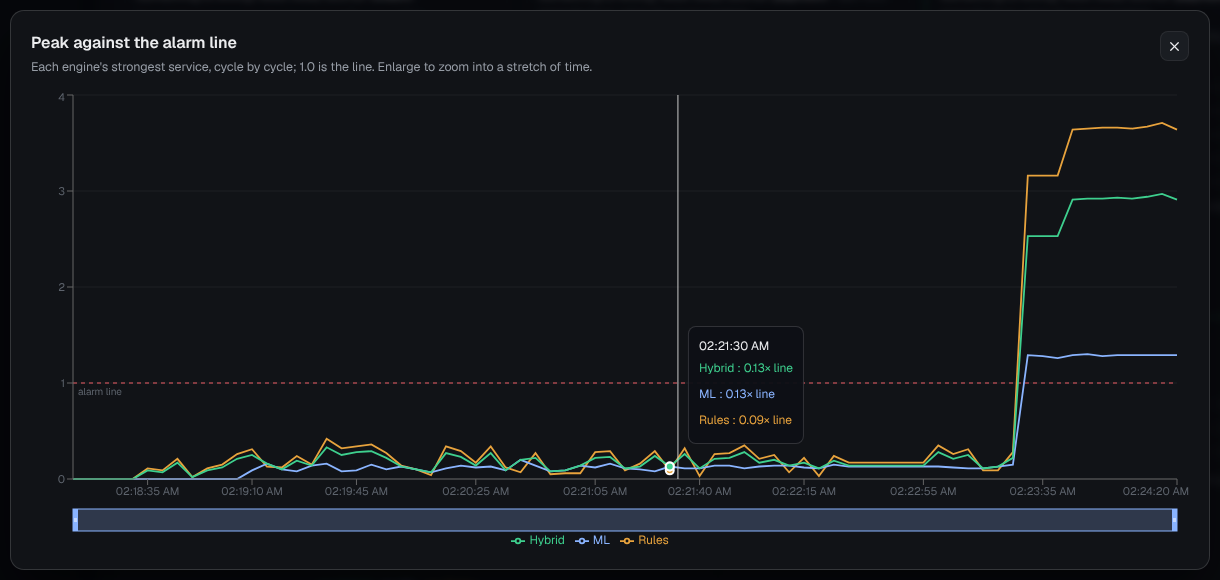
\includegraphics[width=0.9\textwidth]{ui_engines_popup.png}
\caption{An enlarged chart with its time brush and hover read-out.}
\end{figure}

\begin{saybox}
``Look at the pop-up: the rule score climbs higher than the ML peak, but on the wrong service. The ML peak crosses the line once and stays just above it, on the right service. That is the whole difference between the engines, on one chart.''
\end{saybox}

\begin{warnbox}
In the demo on the simulator, the ML engine alarms on the slow \code{payment} fault and then, after about 48 simulated seconds, absorbs it and goes quiet (its two-minute drift rule). The Rules and Hybrid engines keep alarming. If someone asks why ML went quiet, that is the answer, and it is in the limitations.
\end{warnbox}

\section{Cascade risk}
\begin{figure}[H]
\centering
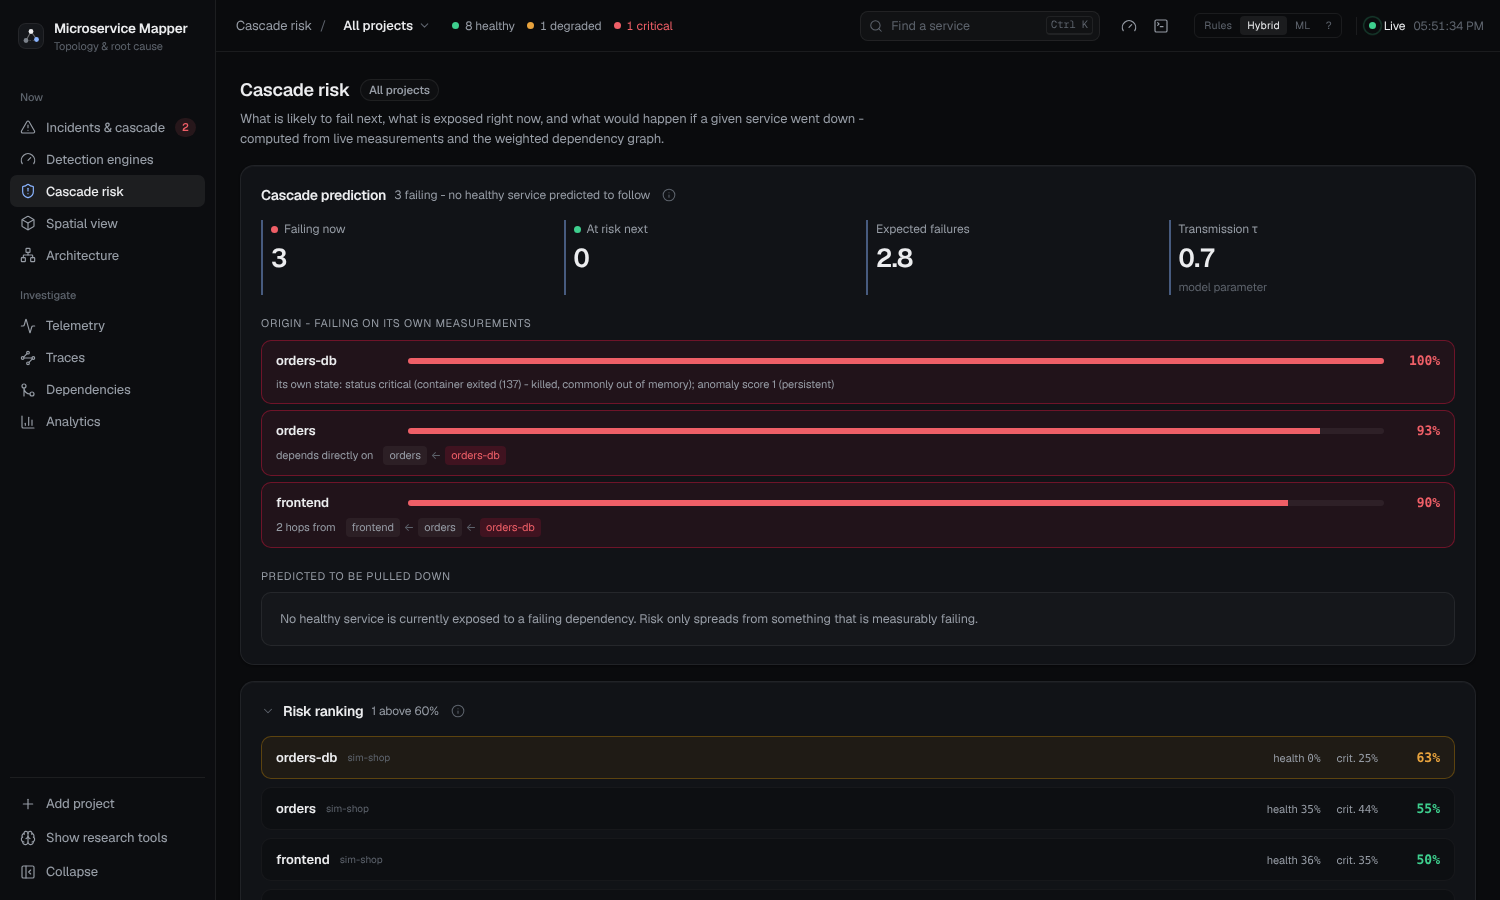
\includegraphics[width=0.96\textwidth]{ui_cascade_risk_fault.png}
\caption{Cascade risk during the fault.}
\end{figure}
\begin{simplebox}
Three questions in one page: what is failing now (judged on its own measurements), what is exposed (which services have a lot depending on them), and what would happen if a chosen service failed (what-if). Every prediction shows the \emph{name of the model and its parameter} beside it. No bare numbers.
\end{simplebox}

\section{Telemetry, Traces, Dependencies, Analytics}
\begin{figure}[H]
\centering
\setlength{\tabcolsep}{2pt}
\begin{tabular}{cc}
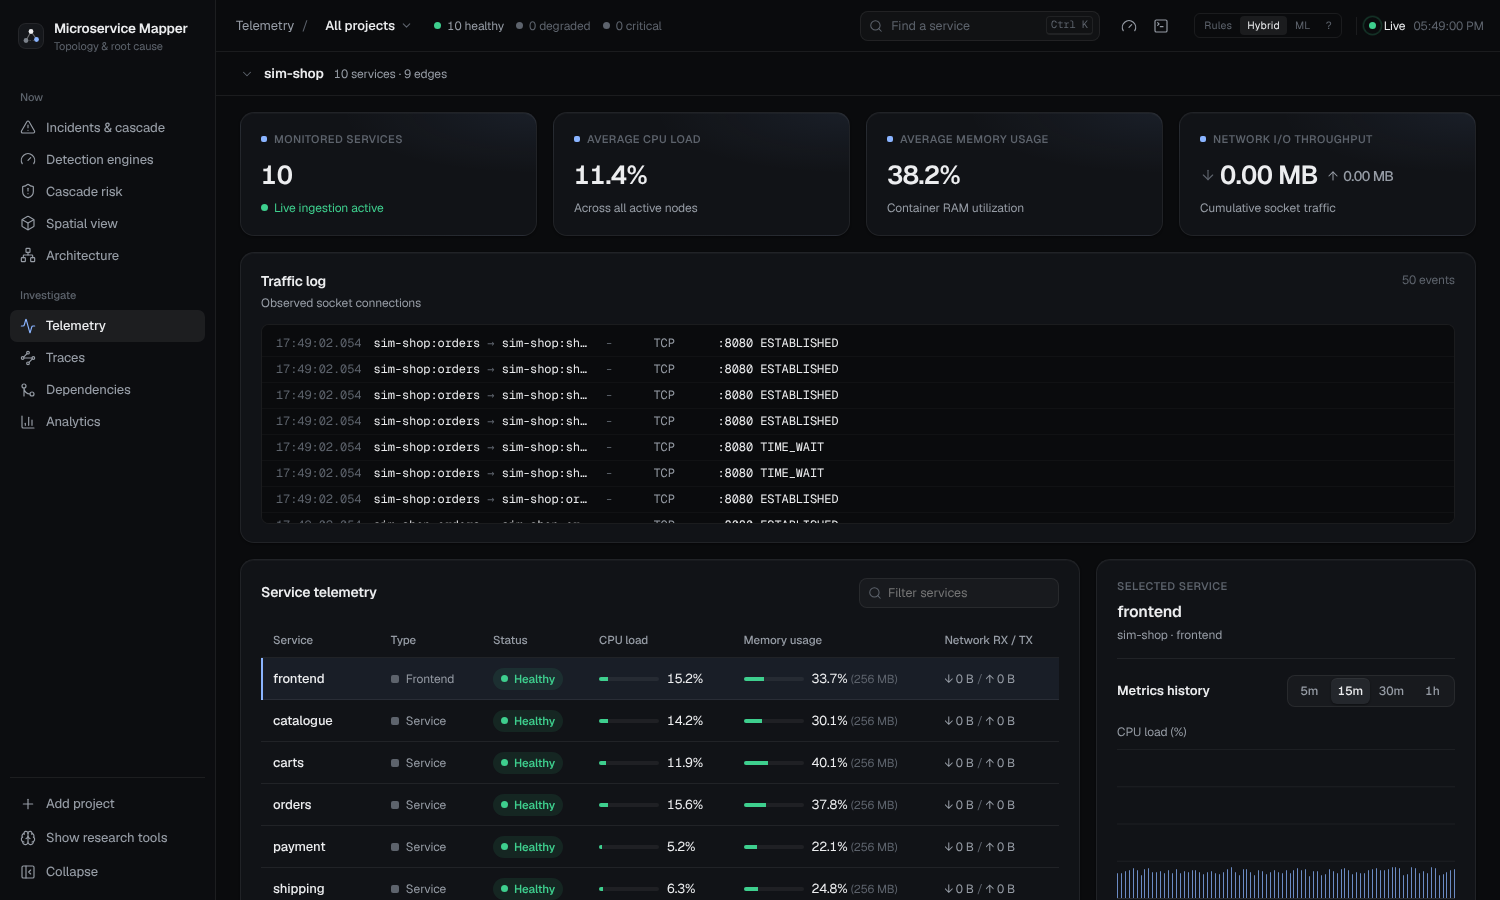
\includegraphics[width=0.49\textwidth]{ui_telemetry.png} & 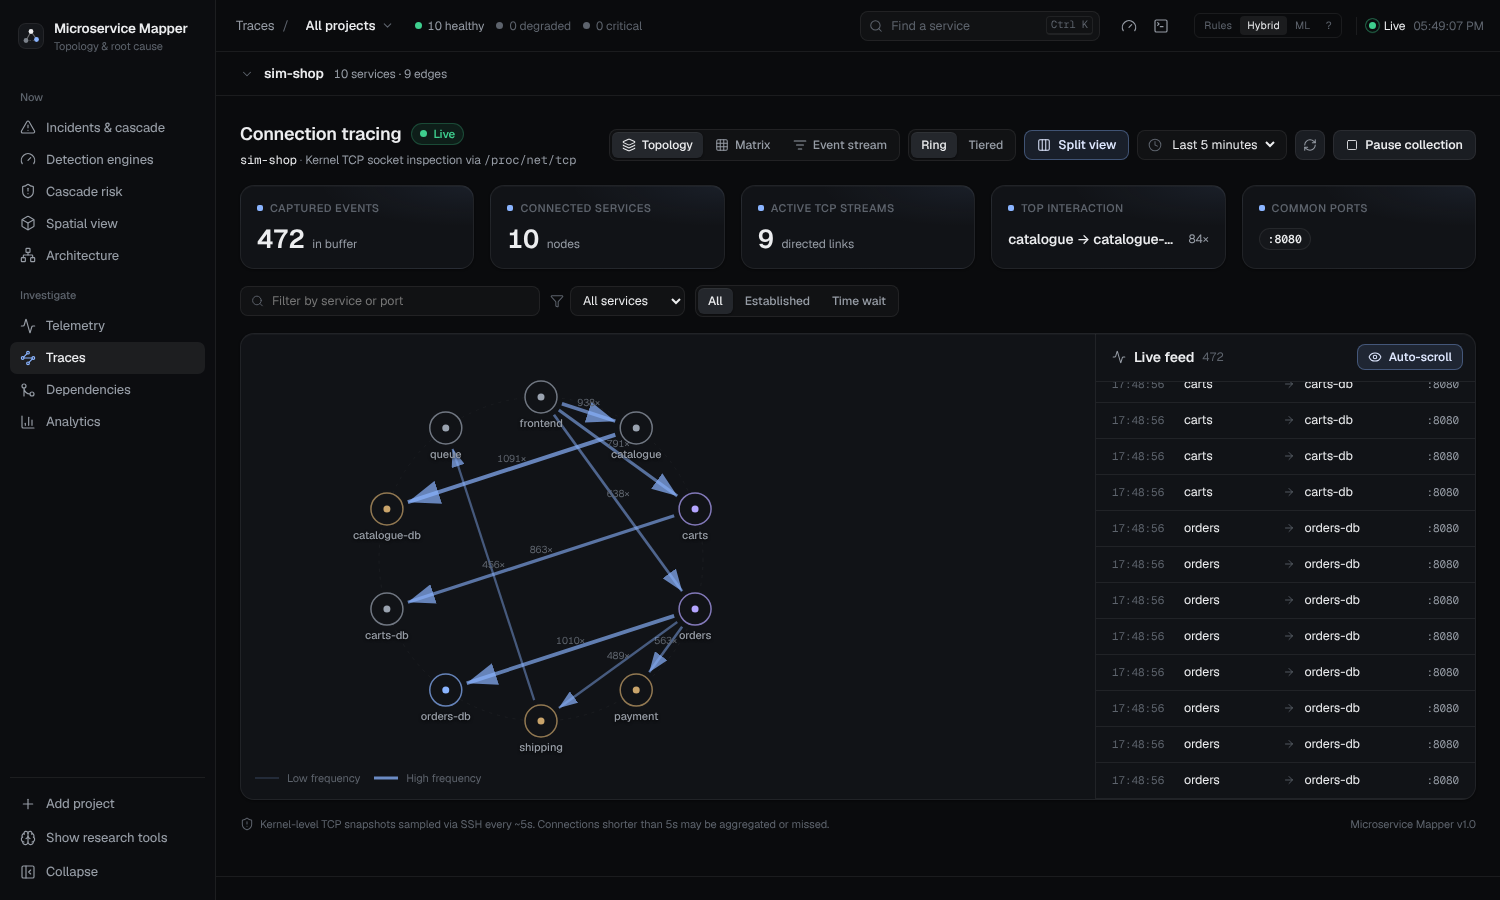
\includegraphics[width=0.49\textwidth]{ui_traces.png}\\
\small (a) Telemetry & \small (b) Traces\\[4pt]
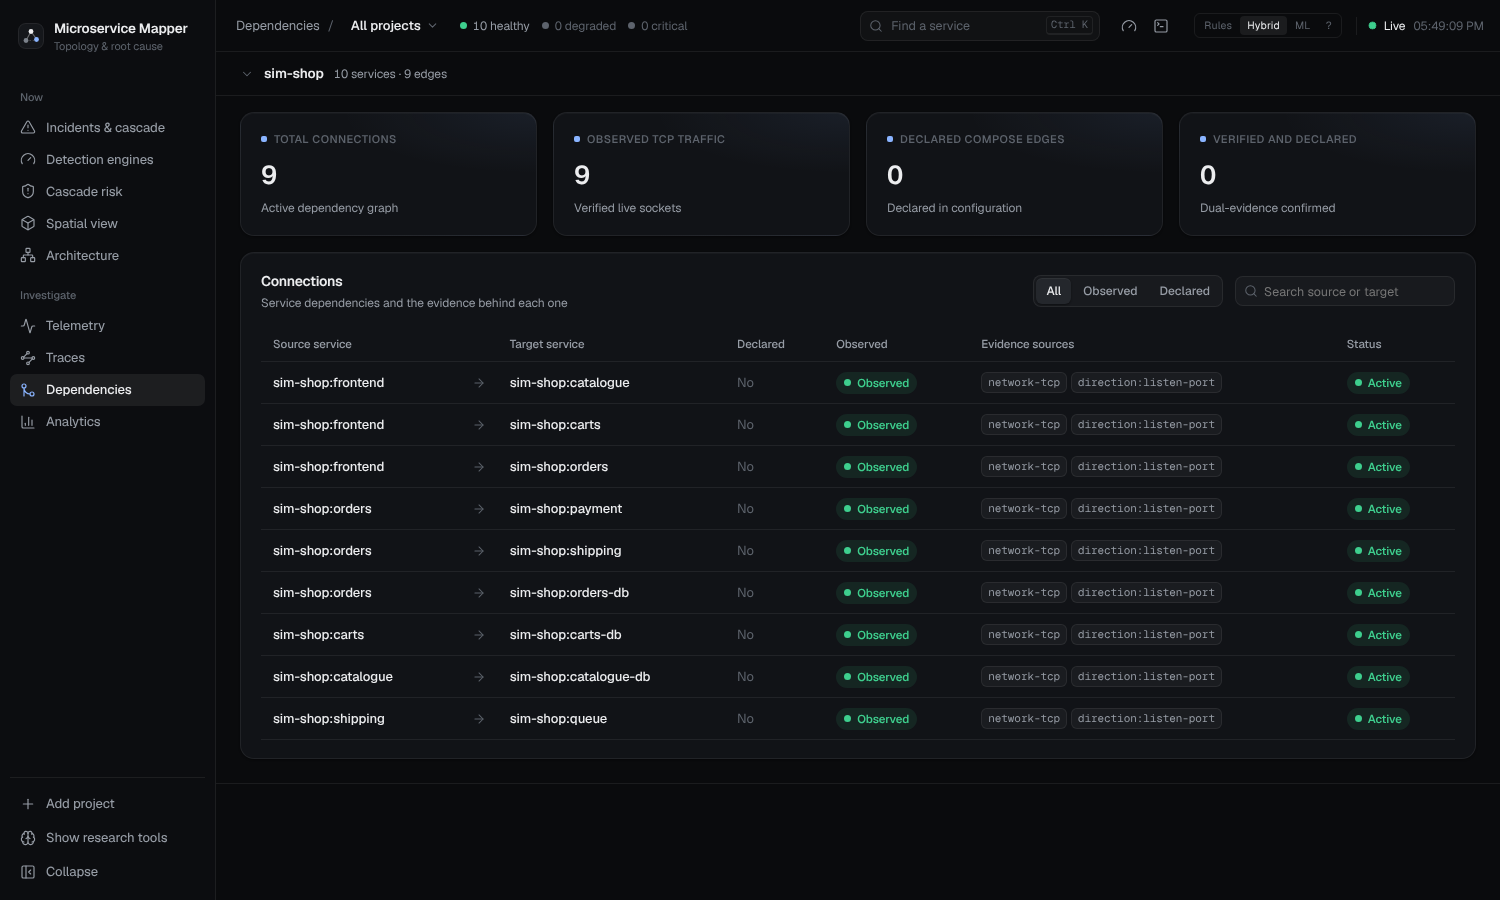
\includegraphics[width=0.49\textwidth]{ui_dependencies.png} & 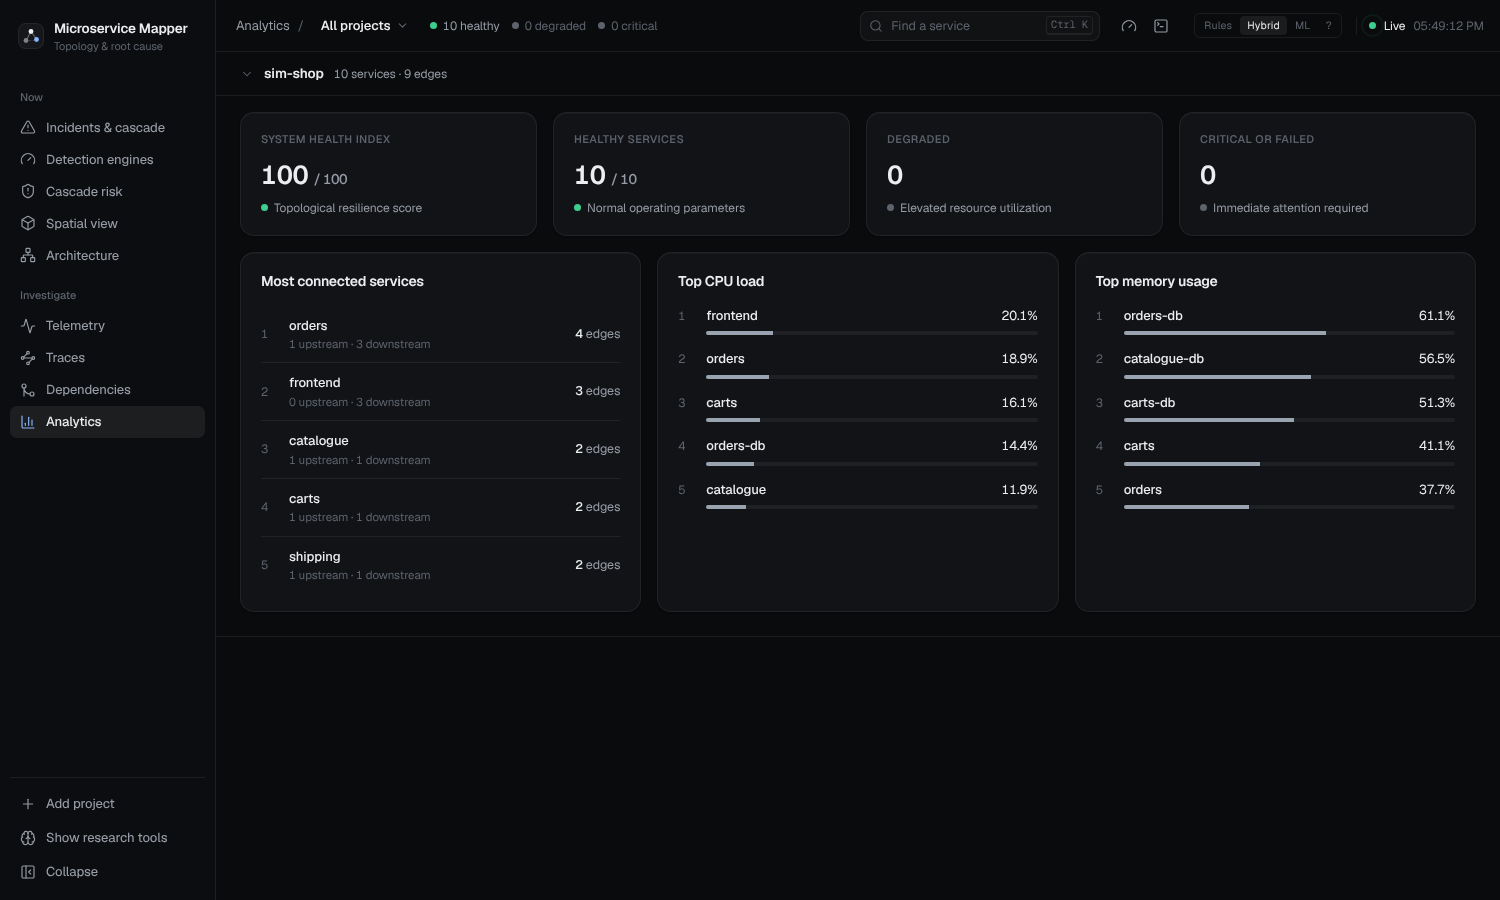
\includegraphics[width=0.49\textwidth]{ui_analytics.png}\\
\small (c) Dependencies & \small (d) Analytics
\end{tabular}
\caption{The investigation pages.}
\end{figure}
\begin{simplebox}
\textbf{Telemetry} is the raw numbers: fleet totals, the live connection log, a sortable per-service table with a history chart. \textbf{Traces} shows sampled connections as a ring, a matrix or an event stream; it is \emph{not} request tracing. \textbf{Dependencies} lists every connection with its declared and observed flags and the evidence sources (for example \emph{network-tcp} and \emph{direction:listen-port}). \textbf{Analytics} gives a health index, the counts of healthy/degraded/critical services, the most connected services and the top CPU and memory users.
\end{simplebox}

\begin{warnbox}
The ``Traces'' page name is a trap. It is not distributed tracing. It is a view of sampled TCP sockets. Say so before an evaluator assumes otherwise.
\end{warnbox}

\section{The 3D spatial view}
\begin{simplebox}
The 3D view draws the same graph as a small city. Services are buildings on platforms. Links are cables: thick cables are heavily used links; the colour shows how healthy the link is; and little pulses move along them faster when the link carries more requests. A card floats over each platform with its role and how many services it holds. A \emph{Cards} button hides the cards when they cover things.

Four arrangements answer four questions:
\begin{itemize}
\item \textbf{Islands}: ``what kinds of services do I have?'' --- one raised platform per role (edge, services, messaging, data).
\item \textbf{Flow}: ``in what order does a request travel?'' --- platforms in order from entry points to data, with a note on how many callers a fault at each hop can reach.
\item \textbf{Topology}: ``what would hurt the most if it broke?'' --- services grouped by how much depends on them.
\item \textbf{Tiers}: ``are my layers respected?'' --- layers stacked as terraces from edge down to data; a call that skips a layer or goes up the stack stands out.
\end{itemize}
\end{simplebox}

\begin{figure}[H]
\centering
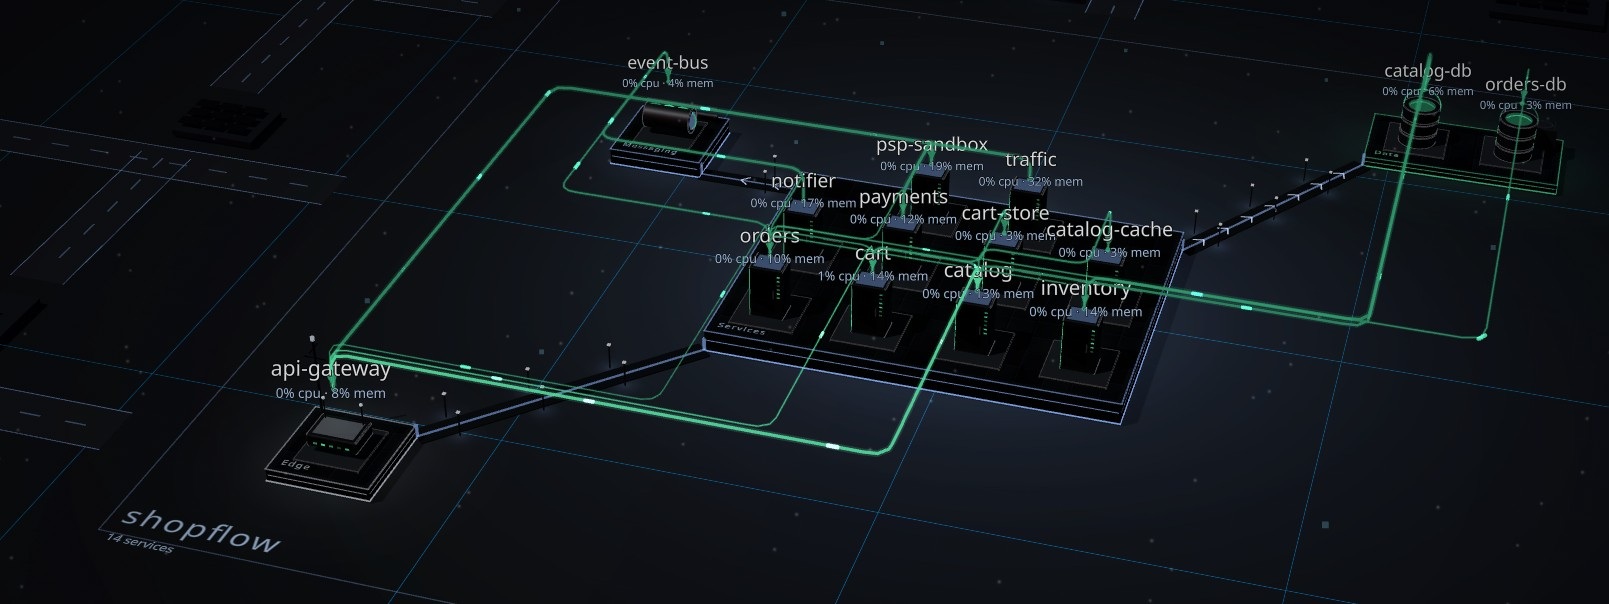
\includegraphics[width=0.84\textwidth]{ui3d_shopflow_islands_nocards.jpg}\\[3pt]
{\small (a) Islands}\\[6pt]
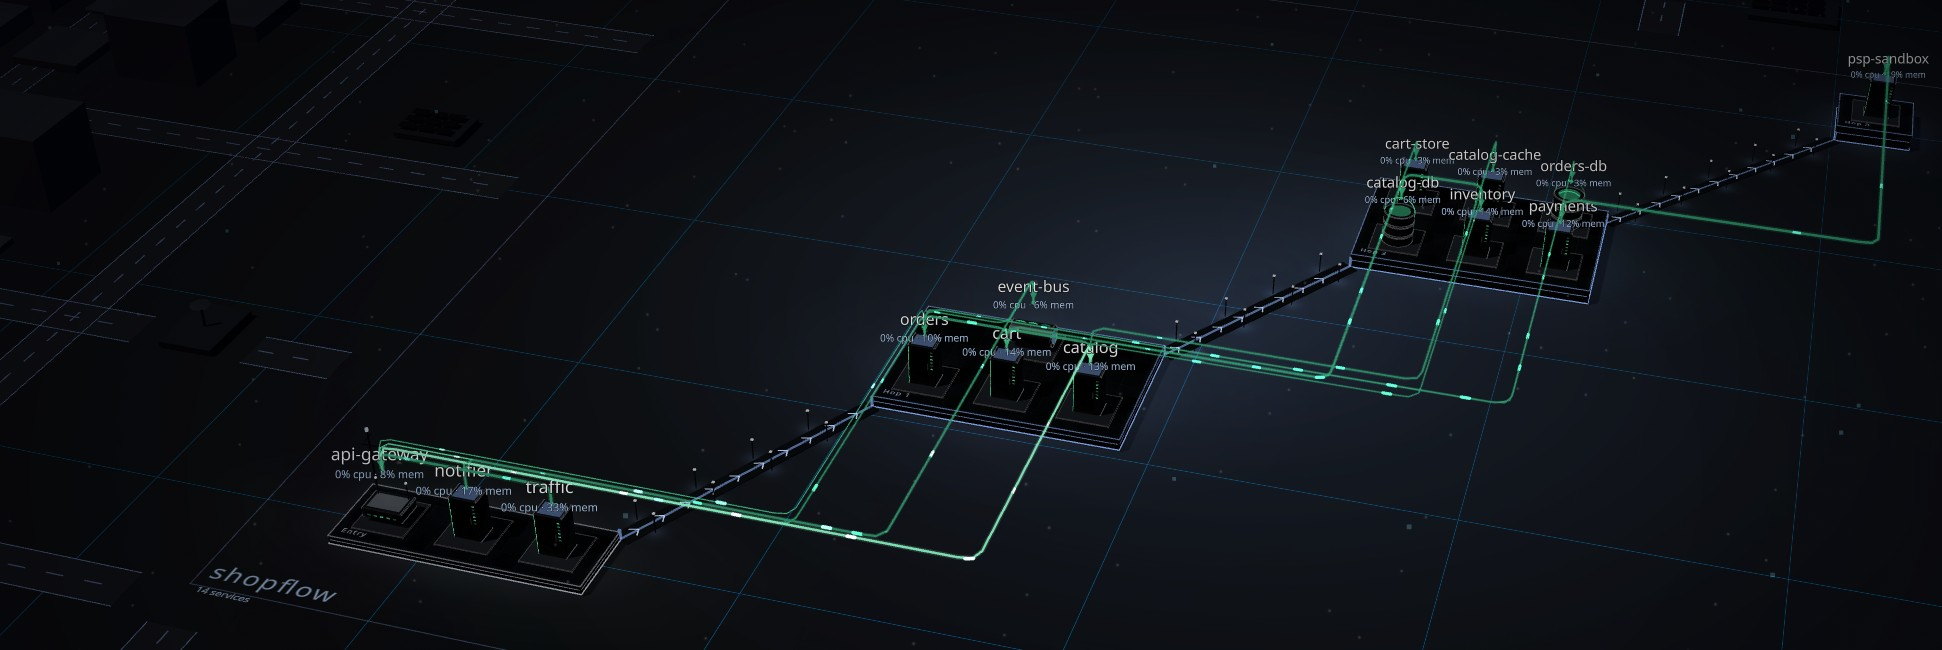
\includegraphics[width=0.84\textwidth]{ui3d_shopflow_flow_nocards.jpg}\\[3pt]
{\small (b) Flow}
\caption{ShopFlow in two of the four 3D arrangements.}
\end{figure}
\begin{figure}[H]
\centering
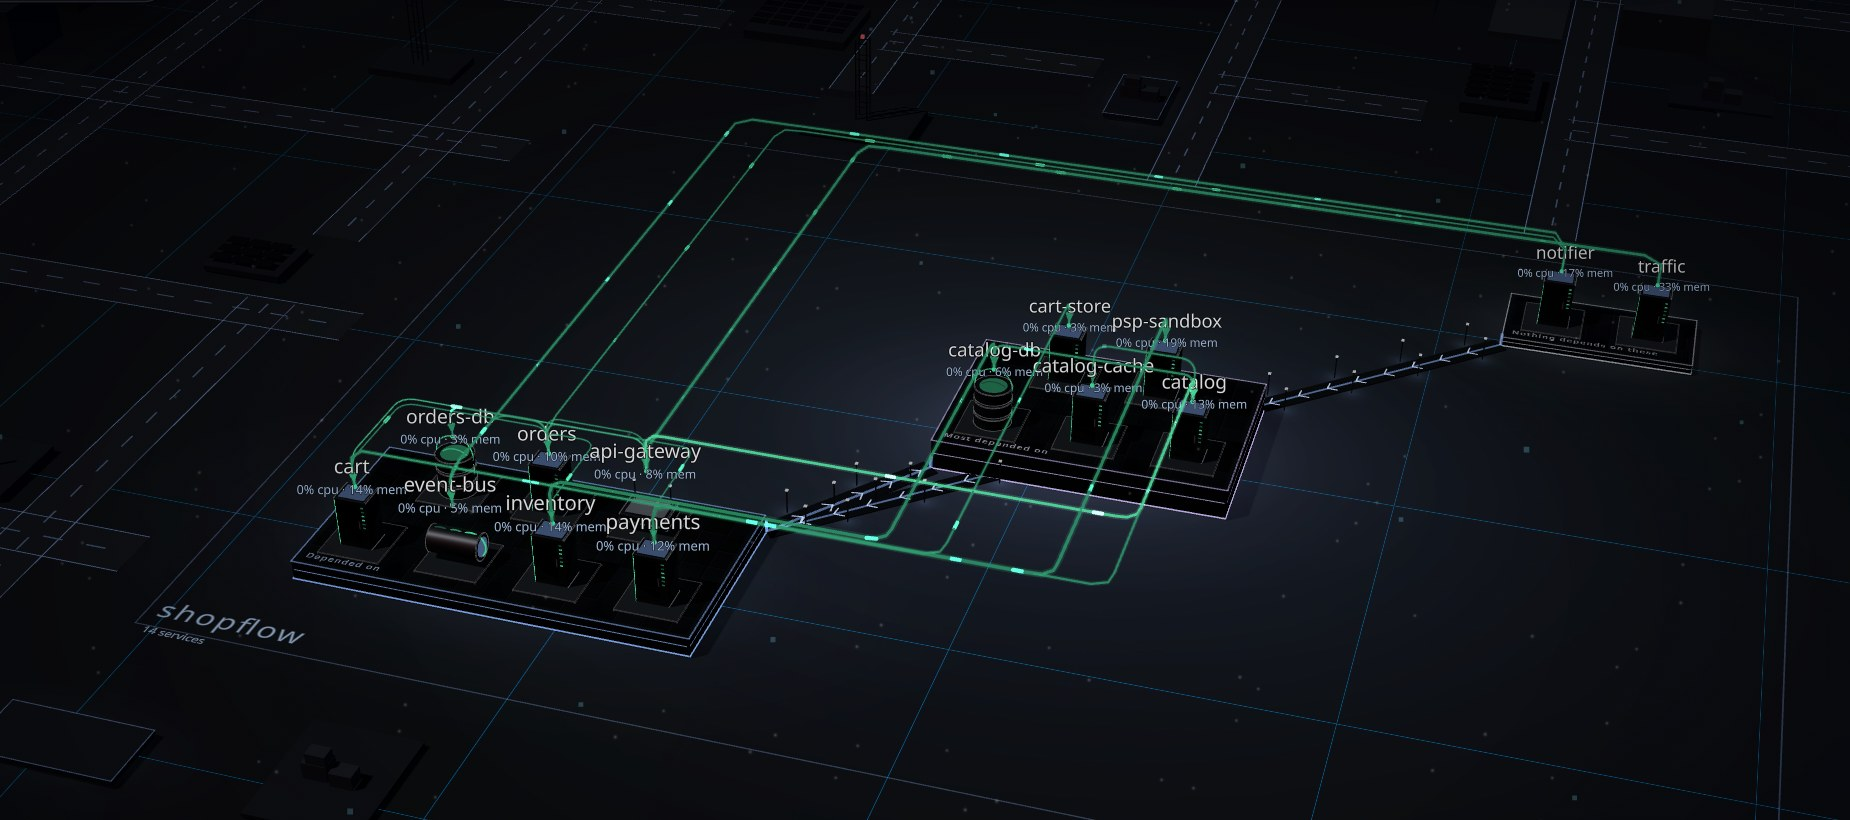
\includegraphics[width=0.84\textwidth]{ui3d_shopflow_topology_nocards.jpg}\\[3pt]
{\small (c) Topology}\\[6pt]
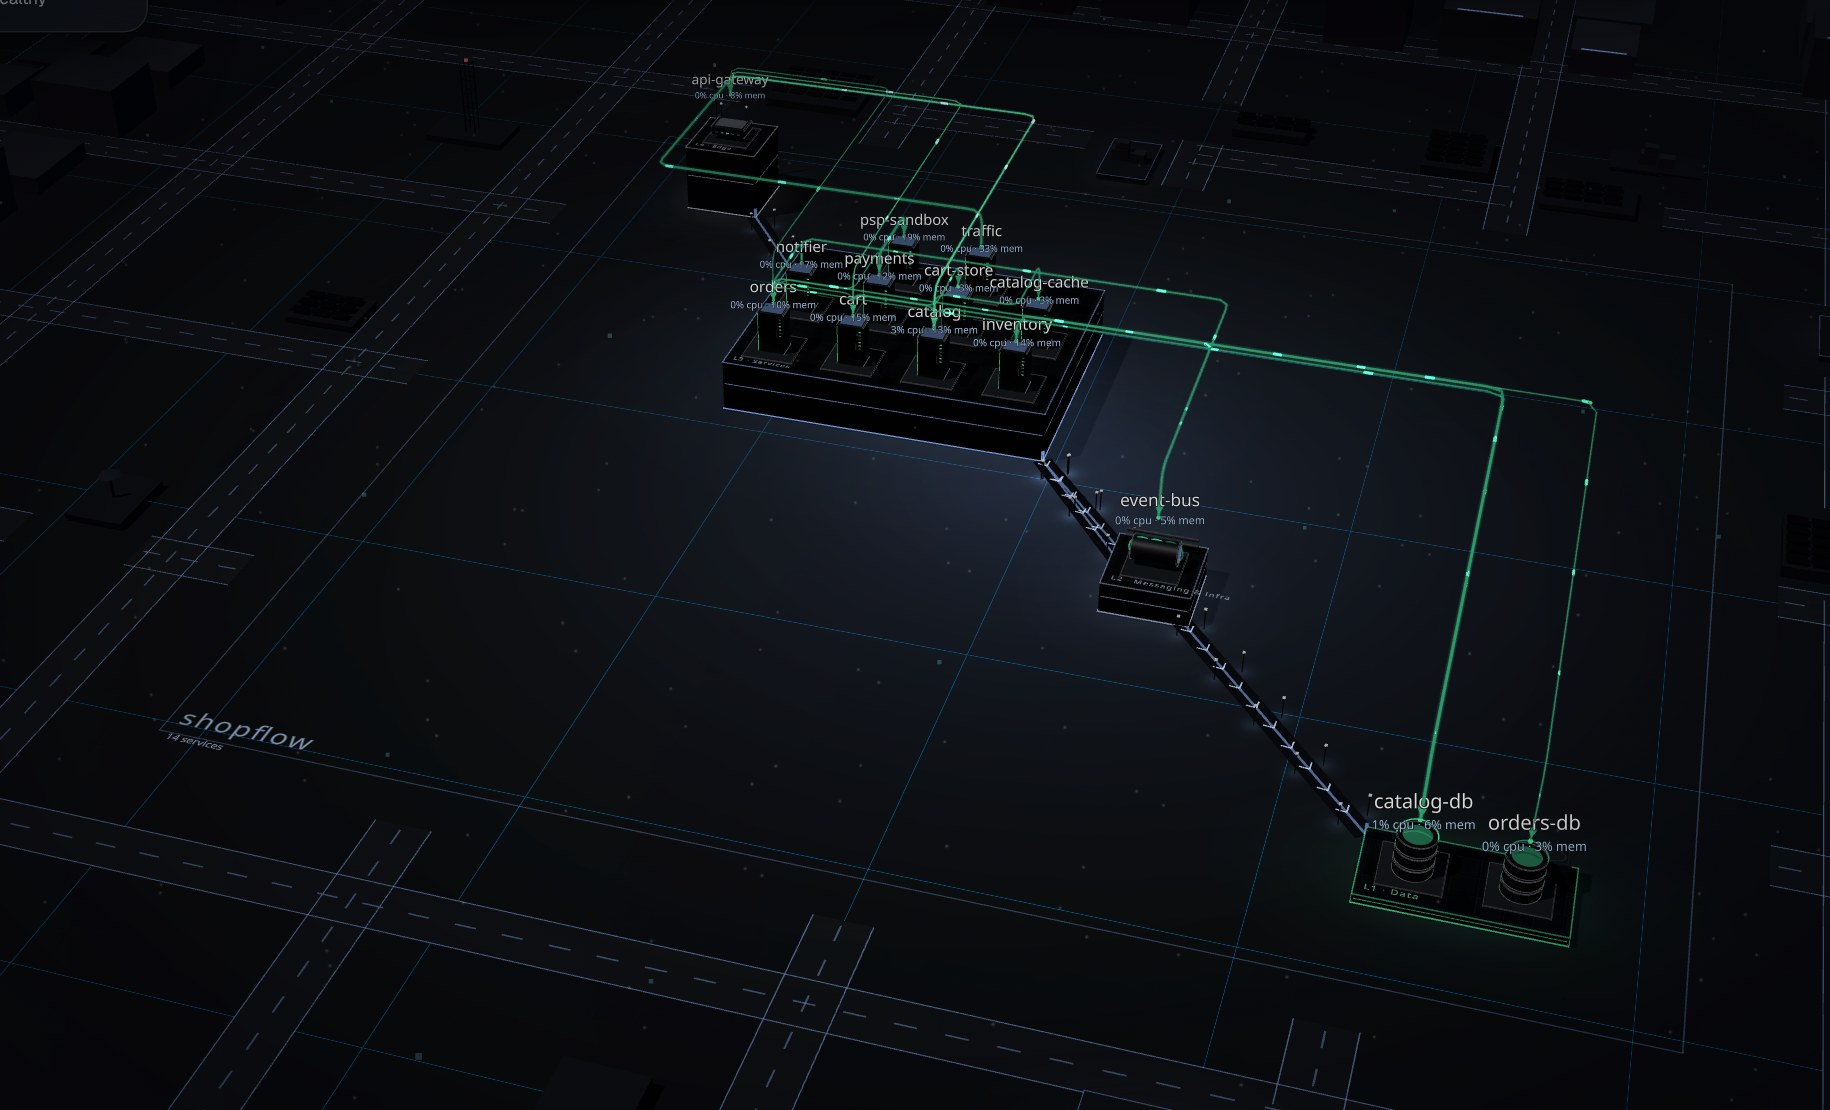
\includegraphics[width=0.62\textwidth]{ui3d_shopflow_tiers_nocards.jpg}\\[3pt]
{\small (d) Tiers}
\caption{ShopFlow in the other two arrangements.}
\end{figure}
\begin{figure}[H]
\centering
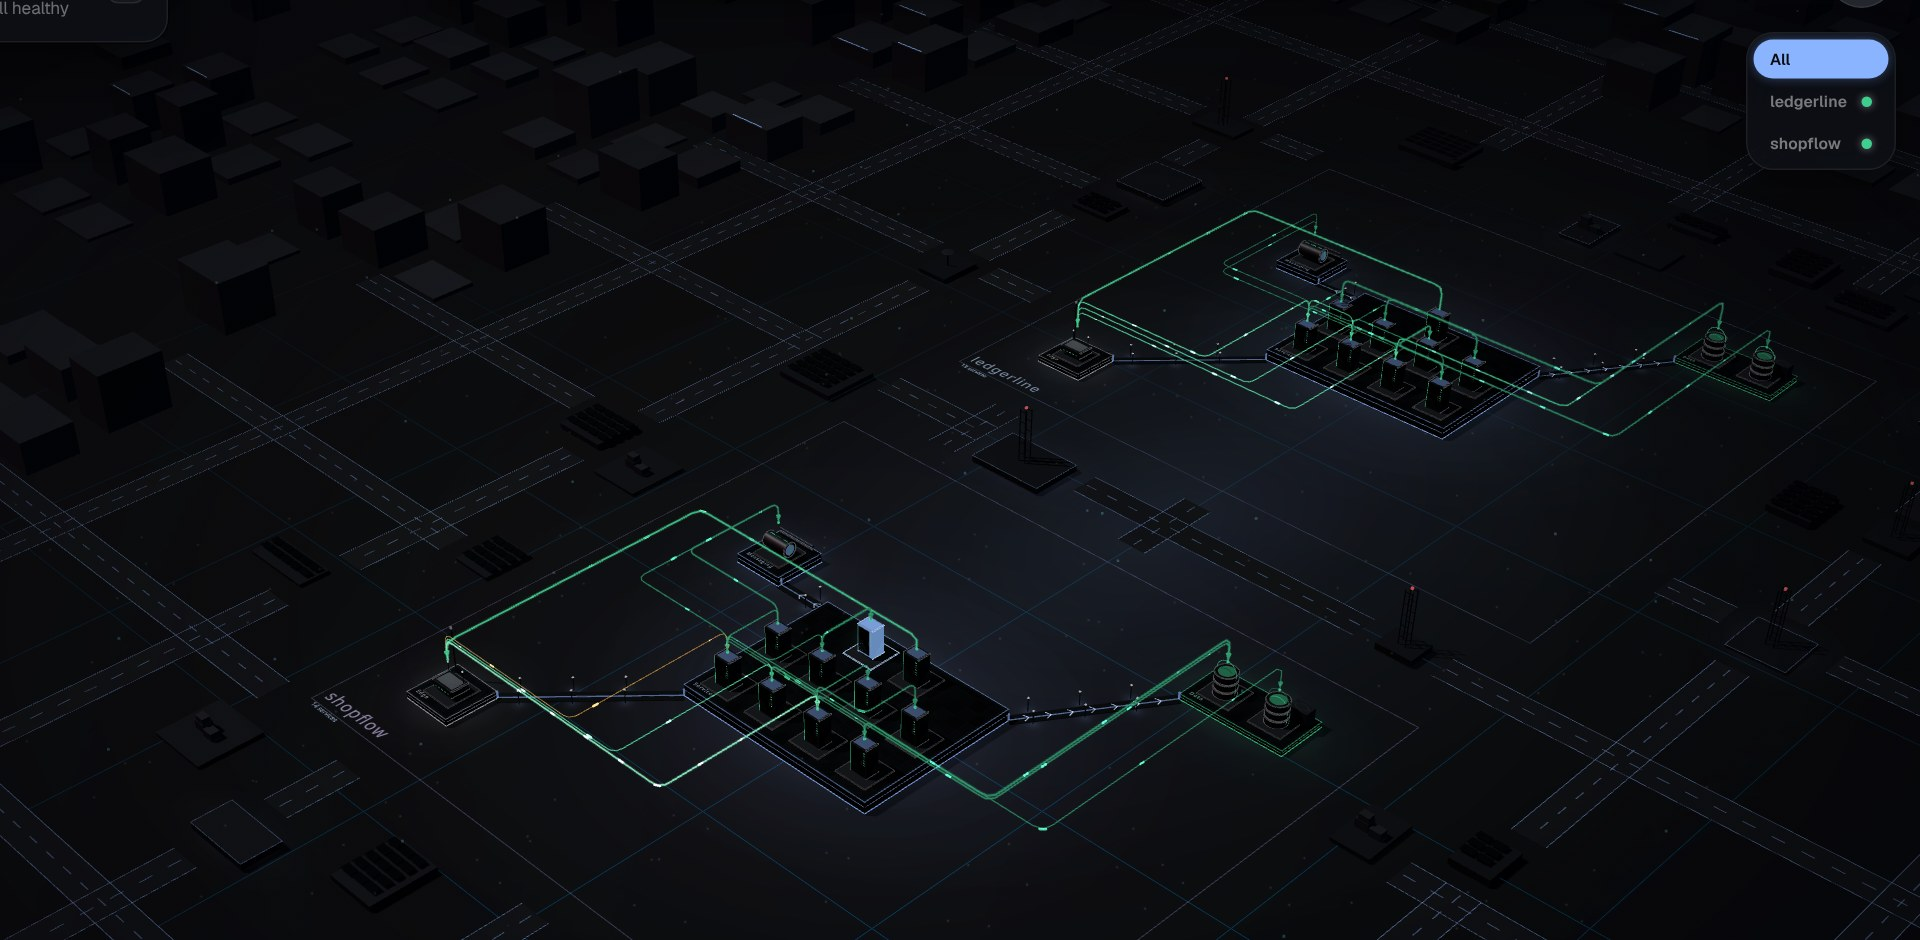
\includegraphics[width=0.9\textwidth]{ui3d_all_nocards.jpg}\\[3pt]
{\small (a) All projects}\\[6pt]
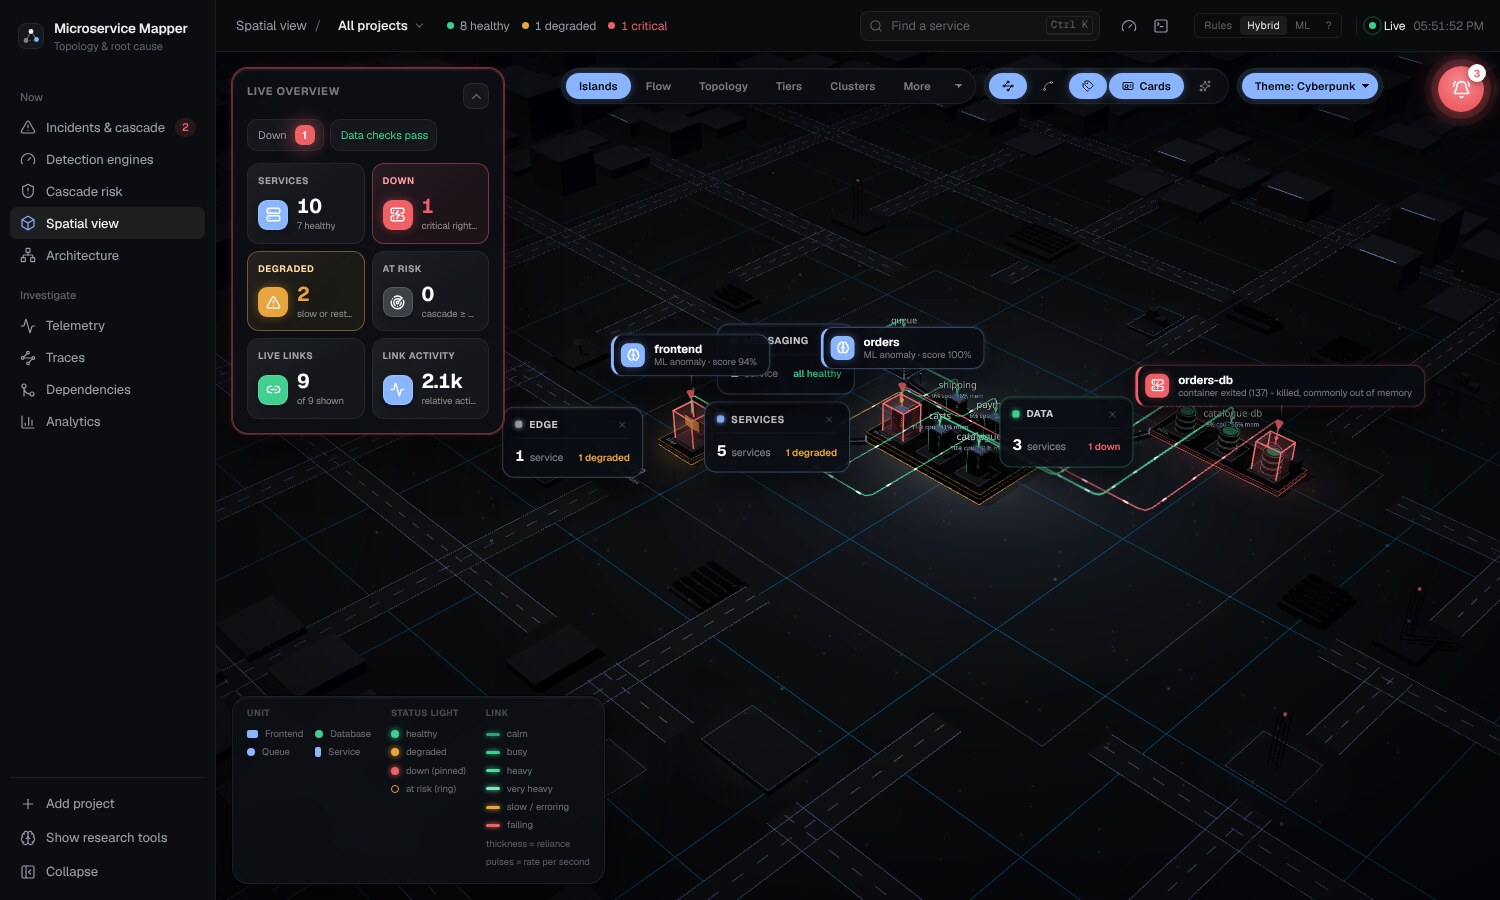
\includegraphics[width=0.9\textwidth]{ui3d_islands_fault.jpg}\\[3pt]
{\small (b) ShopFlow during a fault: \code{payments} paused}
\caption{The Islands view of all projects, and a fault in one of them.}
\end{figure}

\begin{saybox}
``Islands for what we have, Flow for how a request travels, Topology for what hurts most if it breaks, Tiers for whether the layers are respected. During a fault the failing unit is boxed in red with its name and score, and the bell in the corner counts what needs attention.''
\end{saybox}

\begin{techbox}
The scene is built with Three.js through react-three-fiber. Link thickness encodes the dependency weight and colour the heat of the link (calm, busy, heavy, very heavy, slow/erroring, failing); pulse rate is driven by the link's request rate. The legend on screen gives the status lights: green healthy, orange degraded, red down, and a ring for a service the cascade model marks at risk; a unit that the ML engine flags gets a callout with its name and anomaly score. Themes: Cyberpunk, Studio, Hologram. The camera frames the content automatically and flies to a zone or a service when selected.
\end{techbox}
